\documentclass{standalone}
\usepackage{tikz}
\usepackage{ctex,siunitx}
\setCJKmainfont{Noto Serif CJK SC}
\usepackage{tkz-euclide}
\usepackage{amsmath}
\usetikzlibrary{patterns, calc,3d}
\usetikzlibrary {decorations.pathmorphing,decorations.pathreplacing,decorations.shapes}
\begin{document}
\small
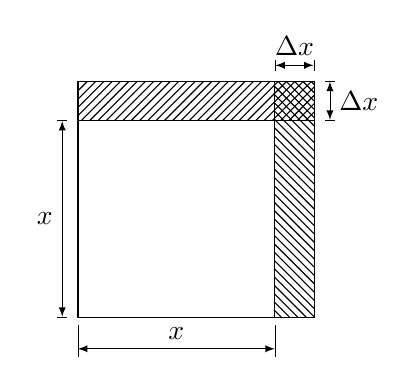
\begin{tikzpicture}[>=latex]
  \draw(0,0)rectangle(2.5,2.5);
  \draw[pattern =north east lines](0,2.5)rectangle(3,3);
  \draw[pattern =north west lines](2.5,0)rectangle(3,3);
  \draw[very thin,|<->|](-0.2,0)--(-0.2,2.5)node[midway,left]{$x$};
  \draw[very thin,|<->|](3.2,2.5)--(3.2,3)node[midway,right]{$\Delta x$};
  \draw[very thin](0,-0.1)--(0,-0.5)(2.5,-0.1)--(2.5,-0.5);
  \draw[very thin,<->](0,-0.4)--(2.5,-0.4)node[midway,above]{$x$};
  \draw[very thin,|<->|](2.5,3.2)--(3,3.2)node[midway,above]{$\Delta x$};
\end{tikzpicture}
\end{document}